\documentclass{article}

\usepackage[letterpaper]{geometry}
\usepackage{amsmath}
\usepackage{amssymb}
\usepackage{siunitx}
\usepackage{graphicx}
\usepackage{minted}
\usepackage{tikz}
\usepackage{minted}
%\usepackage{gnuplot-lua-tikz}

\title{4125 HW 7}
\author{Duncan Wilkie}
\date{27 April 2022}

\begin{document}

\maketitle

\section*{6.5a}
Applying the definition,
\[
  Z=\sum_{s}e^{-E(s)/kT}=e^{(\SI{-0.05}{eV})(\SI{1.6e-19}{J/eV})/(\SI{1.38e-23}{J/K})(\SI{300}{K})}
  +e^{0}
\]
\[
  +e^{(\SI{0.05}{eV})(\SI{1.6e-19}{J/eV})/(\SI{1.38e-23}{J/K})(\SI{300}{K})}
\]
\[=8.05\]

\section*{6.5b}
The Boltzmann distribution is
\[P(s)=\frac{1}{Z}e^{-E(s)/kT}\]
Applying it,
\[P(\SI{-0.05}{eV})=\frac{1}{8.05}e^{(\SI{0.05}{eV})(\SI{1.6e-19}{J/eV})/(\SI{1.38e-23}{J/K})(\SI{300}{K})}=0.86\]
\[P(\SI{0}{eV})=\frac{1}{8.05}e^{0}=0.12\]
\[O(\SI{0.05}{eV})=\frac{1}{8.05}e^{-(\SI{0.05}{eV})(\SI{1.6e-19}{J/eV})/(\SI{1.38e-23}{J/K})(\SI{300}{K})}=0.018\]

\section*{6.5c}
Doing the same calculation,
\[Z=e^{0}+e^{-(\SI{0.05}{eV})(\SI{1.6e-19}{J/eV})/(\SI{1.38e-23}{J/K})(\SI{300}{K})}\]
\[+e^{-(\SI{0.1}{eV})(\SI{1.6e-19}{J/eV})/(\SI{1.38e-23}{J/K})(\SI{300}{K})}=1.17\]
\[P(\SI{0}{eV})=\frac{1}{Z}e^{0}=0.86\]
\[P(\SI{0.05}{eV})=\frac{1}{1.17}e^{-(\SI{0.05}{eV})(\SI{1.6e-19}{J/eV})/(\SI{1.38e-23}{J/K})(\SI{300}{K})}=0.12\]
\[P(\SI{0.1}{eV})=\frac{1}{1.17}e^{-(\SI{0.1}{eV})(\SI{1.6e-19}{J/eV})/(\SI{1.38e-23}{J/K})(\SI{300}{K})}=0.018\]
The partition function changes, but the probabilities don't.
Numerically verifying something whose proof is obvious and is given in the text is pure torture.

\section*{6.13}
The difference in energy is
\[\Delta E=\Delta m c^{2}=(\SI{2.3e-30}{kg})(\SI{3e8}{m/s})^{2}=\SI{2.07e-13}{J}\]
The ratio of the probability of a particle being in one state to that of the other is
\[\frac{P(\textrm{neutron})}{P(\textrm{proton})}=e^{-\Delta E/kT}=e^{-(\SI{2.07e-13}{J})/(\SI{1.38e-23})(\SI{e11}{K})}=0.86\]
We also have $P(\textrm{neutron})+P(\textrm{proton})=1\Leftrightarrow P(\textrm{neutron})=1-P(\textrm{proton})$.
Substituting this,
\[\frac{1}{P(\textrm{proton})}-1=0.86\Rightarrow P(\textrm{proton})=\frac{1}{1+0.86}=0.54\]
\[\Rightarrow P(\textrm{neutron})=1-0.54=0.46\]
These will be the fractions of the nucleons that are of each type of particle, respectively.

\section*{6.15a}
\[\overline{E}=[4(\SI{0}{eV})+3(\SI{1}{eV})+2(\SI{4}{eV})+1(\SI{6}{eV})]/10=\SI{1.7}{eV}\]

\section*{6.15b}
For $\SI{0}{eV}$, it's $4/10=0.4$; for $\SI{1}{eV}$, it's $3/10=0.3$; for $\SI{4}{eV}$, it's $2/10=0.2$; for $\SI{6}{eV}$, it's $1/10=0.1$.

\section*{6.15c}
Applying the formula,
\[\overline{E}=0.4(\SI{0}{eV})+0.3(\SI{1}{eV})+0.2(\SI{4}{eV})+0.1(\SI{6}{eV})=\SI{1.7}{eV}\]

\section*{6.21}
Using Sage:
\begin{minted}{sage}
|--------------------------------------------------------------------|
| SageMath version 9.2, Release Date: 2020-10-24                     |
| Using Python 3.9.2. Type "help()" to get help.                     |
|--------------------------------------------------------------------|
sage: var('n eps beta T k x')
(n, eps, beta, T, k, x)
sage: E(n) = eps*(1.03*n-0.03*n^2)
sage: Z(beta) = sum(exp(-beta*E), n, 0, 15)
sage: U(beta) = -1/Z(beta)*diff(Z(beta), beta)
sage: C(T) = diff(U(1/(k*T)), T)
sage: C = (C(eps*x/k) / k).full_simplify()
sage: plot(C(x), (x, 0, 3))
# Launched png viewer for Graphics object consisting of 1 graphics primitive
\end{minted}
This produces the following plot of the heat capacity
\[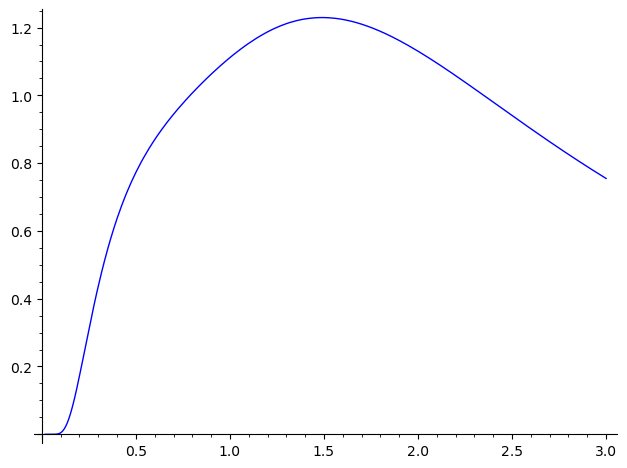
\includegraphics[scale=0.8]{cap.png}\]
where the vertical axis is $C/k$ and the horizontal is $kT/\epsilon$ (couldn't be bothered to figure out TeX formatting of plot fields in Sage).
Including fewer levels results in a faster falloff on the right side of the graph.
In the case of the harmonic oscillator, the heat capacity doesn't actually fall off at large $T$, but approaches a constant value.
The vibrational portion of figure 1.13 is more consistent with this anharmonic model, as it doesn't appear to level off as $T$ increases.

\section*{6.26}
The approximate partition function is
\[Z_{rot}=1+3e^{-2\epsilon/kT}\]
The average energy is then
\[
  \overline{E}=\frac{1}{Z}\sum_{j=0}^{1}E(j)(2j+1)e^{-E(j)/kT}
  =\frac{1}{1+3e^{-2\epsilon/kT}}\left( 0+6\epsilon e^{-2\epsilon/kT} \right)
  \approx 6\epsilon e^{-2\epsilon/kT}
\]
The heat capacity is
\[
  C_{V}=\frac{\partial\overline{E}}{\partial T}
  =\frac{12\epsilon^{2}}{kT^{2}}e^{-2\epsilon/kT}
\]
The relationship between heat capacity and entropy yields
\[
  \frac{{C_{V}}}T=\frac{\partial S}{\partial T}
  \Rightarrow S=\frac{12\epsilon^{2}}{k}\int\frac{e^{-2\epsilon/kT}}{T^{3}}dT
\]
In the limit as $T\to 0$, the numerator of the integrand will fall to zero much faster than the denominator, so this result is consistent
with the third law of thermodynamics.
The high-temperature limit is a constant, so a simple interpolation between them would be a function that's roughly $e^{-1/T}$ in the
limit to zero and constant in the limit to infinity, as shown below.
\[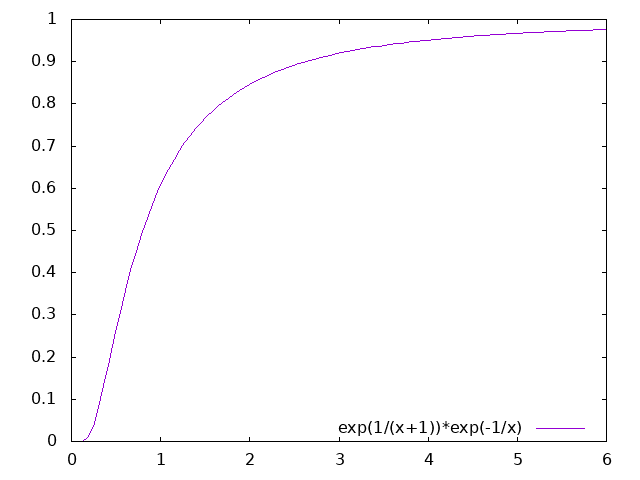
\includegraphics[scale=0.8]{plot3.png}\]

\section*{6.32a}
For a continuous probability distribution $P(x)$ the expectation value of $x$ is
\[\langle x \rangle = \int_{\mathbb{R}}xP(x)dx\]
In the case of a particle in a potential well, the probability of the particle being in the position $x$ is
\[P(x)=\frac{e^{-\beta u(x)}}{Z}\]
since the energy state of the particle is determined by its position according to $u$.
Applying the definition of the partition function and writing the sum over an uncountably infinite index as an integral,
\[\langle x \rangle = \int_{\mathbb{R}}x\frac{e^{-\beta u(x)}}{\int_{\mathbb{R}}e^{-\beta u(x)}dx}dx\]
Factoring out the constant,
\[\langle x \rangle=\frac{\int_{\mathbb{R}}xe^{-\beta u(x)}dx}{\int_{\mathbb{R}}e^{-\beta u(x)}dx}\]
as desired.

\section*{6.32b}
If $x_{0}$ is the minimum of the potential, then it must also be a critical point, i.e. $\frac{du}{dx}\big|_{x_{0}}=0$.
Plugging the approximation
\[ u(x)=u(x_{0})+\frac{1}{2}(x-x_{0})^{2}\frac{d^{2}u}{dx^{2}}\bigg|_{x_{0}}\]
into the above-derived expression for the expectation of position,
\[
  \langle x \rangle=\frac{e^{-\beta u(x_{0})}}{e^{-\beta u(x_{0})}}\frac{\int_{\mathbb{R}}xe^{-\beta \frac{u''(x_{0})}{2}(x-x_{0})^{2}}dx}
  {\int_{\mathbb{R}}e^{-\beta \frac{u''(x_{0})}{2}(x-x_{0})^{2}}dx}
  =\frac{\int_{\mathbb{R}}(x+x_{0})e^{-ax^{2}}dx}{\int_{\mathbb{R}}e^{-ax^{2}}dx}
\]
Distributing in the numerator will yield an odd function in the first term, which will be zero,
and in the second term everything but $x_{0}$ cancels, leaving $\langle x \rangle = x_{0}$ as desired.

\section*{6.32c}
Proceeding similarly,
\[\langle x \rangle =
  \frac{\int_{\mathbb{R}}xe^{-\beta \frac{u''(x_{0})}{2}(x-x_{0})^{2}}e^{-\beta \frac{u'''(x_{0})}{6}(x-x_{0})^{3}}dx}
  {\int_{\mathbb{R}}e^{-\beta \frac{u''(x_{0})}{2}(x-x_{0})^{2}}e^{-\beta \frac{u'''(x_{0})}{6}(x-x_{0})^{3}}dx}
  \approx \frac{\int_{\mathbb{R}}xe^{-\beta \frac{u''(x_{0})}{2}(x-x_{0})^{2}}
    \left( 1-\left[ \beta\frac{u'''(x_{0})}{6}(x-x_{0})^{3} \right] \right)dx}
  {\int_{\mathbb{R}}e^{-\beta \frac{u''(x_{0})}{2}(x-x_{0})^{2}}
    \left( 1-\left[ \beta\frac{u'''(x_{0})}{6}(x-x_{0})^{3} \right] \right)dx}
\]
\[
  =\frac{\int_{\mathbb{R}}x_{0}e^{-\beta\frac{u''(x_{0})}{2}x^{2}}dx-\int_{\mathbb{R}}(x+x_{0})e^{-\beta\frac{u''(x_{0})}{2}x^{2}}
    \left(\beta\frac{u'''(x_{0})}{6}x^{3}  \right)dx}
  {\int_{\mathbb{R}}e^{-\beta\frac{u''(x_{0})}{2}x^{2}}dx-\int_{\mathbb{R}}e^{-\beta\frac{u''(x_0)}{2}x^{2}}\beta\frac{u'''(x_{0})}{2}x^{3}dx}
\]
\[
  = \frac{x_{0}\sqrt{\frac{2\pi}{\beta u''(x_{0})}}-\frac{\beta u'''(x_{0})}{6}\int_{-\infty}^{\infty}x^{4}e^{-\beta\frac{u''(x_{0})}{2}x^{2}}dx}
  {\sqrt{\frac{2\pi}{\beta u''(x_{0})}}}
\]
\[
  =x_{0}-\frac{\beta u'''(x_{0})}{6}\sqrt{\frac{\beta u''(x_{0})}{2\pi}}\int_{-\infty}^{\infty}x^{4}e^{-ax^{2}}dx
\]
This integral is in the appendix, and evaluates to $\frac{3\sqrt{\pi}}{4a^{5/2}}$.
We therefore have
\[
  =x_{0}-\frac{\beta u'''(x_{0})}{6}\sqrt{\frac{\beta u''(x_{0})}{2\pi}}\frac{3\sqrt{\pi}}{4\left( \beta u''(x_{0})/2 \right)^{5/2}}
  =x_{0}-\frac{\beta u'''(x_{0})}{8}\sqrt{\frac{\beta u''(x_{0})}{2(\beta u''(x_{0})/2)^{5}}}
  =x_{0}-\frac{\beta u'''(x_{0})}{8}\frac{4}{\beta^{2}u''(x_{0})^{2}}
\]
\[
  =x_{0}-\frac{u'''(x_{0})}{2u''(x_{0})^{2}}\frac{1}{\beta}
\]
Subtracting $x_{0}$ from both sides, this proves that $\langle x \rangle-x_{0}$ is proportional to $kT=\frac{1}{\beta}$
by a proportionality constant
\[-\frac{u'''(x_{0})}{2u''(x_{0})^{2}}\]
In terms of the Taylor coefficients, $u'''(x_{0})=6a_{3}$  and $u''(x_{0})=2a_{2}$, so the proportionality constant may be written
\[
  -\frac{6a_{3}}{8u''(x_{0})^{2}}=-\frac{3a_{3}}{4a_{2}^{2}}
\]

\section*{6.32d}
This potential with $y$-axis in units of $u_{0}$ and $x_{0}=10$ is plotted below.
\[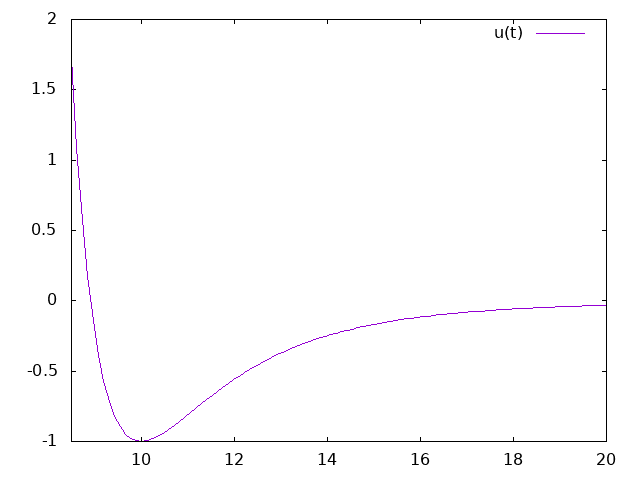
\includegraphics[scale=0.8]{plot.png}\]
The minimum occurs at
\[
  u'(x)=0
  \Leftrightarrow 12u_{0}\left[\frac{x_{0}^{6}}{x^{7}} -\frac{x_{0}^{12}}{x^{13}} \right]=0
  \Leftrightarrow x^{6}=x_{0}^{6}
  \Leftrightarrow x=x_{0}
\]
We only need the two derivatives
\[
  u''(x_{0})=12u_{0}\left[ 13\frac{x_{0}^{12}}{x_{0}^{14}}-7\frac{x_{0}^{6}}{x_{0}^{8}} \right]
  =\frac{72u_{0}}{x_{0}^{2}}
\]
and
\[
  u'''(x_{0})=12u_{0}\left[7\cdot 8\frac{x_{0}^{6}}{x_{0}^{9}} -13\cdot 14\frac{x_{0}^{12}}{x_{0}^{15}} \right]
  =-\frac{1512u_{0}}{x_{0}^{3}}
\]
to compute the proportionality constant
\[
  -\frac{u'''(x_{0})}{2u''(x_{0})^{2}}=\frac{1512u_{0}/x_{0}^{3}}{2\cdot 72^{2}u_{0}^{2}/x_{0}^{4}}
  =\frac{7x_{0}}{48u_{0}}
\]
This proportionality constant is equal to $\alpha x_{0}/k$, since the derivative of the average linear interatomic spacing with respect
to temperature is $k$ times this proportionality constant, and we must divide by the initial spacing to obtain the formula for $\alpha$.
Computing $\alpha$ with the given numbers,
\[
  \alpha=k\frac{7}{48u_{0}}=(\SI{1.38e-23}{J/K})\frac{7}{48(\SI{0.01}{eV})}=\SI{0.0013}{}
\]
which is roughly twice the measured value (possibly due to our assumption of $x_{0}$ as the initial length;
this number would likely agree better if one multiplied it by the ratio $x_{0}/x_{m}$ where $x_{m}$ is the measured interatomic spacing
at $\SI{80}{K}$).

\section*{6.38}
Using the change of variables given in the book to simplify the integral of the Maxwell distribution,
\[x_{min}=v_{min}\sqrt{m/2kT}=(\SI{300}{m/s})\sqrt{(\SI{28}{amu})(\SI{1.66e-27}{kg/amu})/2(\SI{1.38e-23}{J/K})(\SI{300}{K})}\]
\[=0.71\]
The integral corresponding to the proportion of the particles above $\SI{300}{m/s}$ is then, following the text,
\[\frac{4}{\sqrt{\pi}}\int_{0.71}^{\infty}x^{2}e^{-x^{2}}=\frac{4}{\sqrt{\pi}}(0.35)=0.79\]
The proportion below $\SI{300}{m/s}$ is one minus this number, or $0.21$

\section*{6.42a}
The result for one oscillator is immediate:
\[
  F=-kT\ln Z=-kT\ln\left( \frac{1}{1-e^{-\beta\epsilon}} \right)
  =kT\ln\left( 1-e^{-\beta\epsilon} \right)
\]
The Helmholtz free energy is extensive, so if we have $N$ oscillators at the same frequency, the expression is
\[
  F=NkT\ln\left( 1-e^{-\epsilon/kT} \right)
\]

\section*{6.42b}
Applying the partial derivative relation between entropy and Helmholtz free energy,
\[
  S=-\left( \frac{\partial F}{\partial T} \right)_{N,V}
  =-\left( Nk\ln\left(1-e^{-\epsilon/kT}  \right)-NkT\frac{1}{1-e^{-\epsilon/kT}}\frac{\epsilon e^{-\epsilon/kT}}{kT^{2}} \right)
\]
\[
  =N\left( \frac{\epsilon}{Te^{\epsilon/kT}-T}-k\ln\left( 1-e^{-\epsilon/kT} \right) \right)
\]

\section*{6.49}
The volume of the gas is, by the ideal gas law,
\[V=\frac{nRT}{P}=\frac{(\SI{1}{mol})(\SI{8.31}{J/mol\cdot K})(\SI{300}{K})}{\SI{1e5}{Pa}}=\SI{0.025}{m^{3}}\]

We have
\[U=U_{int}+\frac{3}{2}nRT\]
In our case, $kT$ is higher than $\epsilon$ by roughly a factor of 100, so the high temperature limit may be used to calculate $U_{int}$.
The average rotational energy calculation at high temperature performed in the book yields for identical atoms $kT$ per molecule,
implying the total internal energy in the gas is $nRT$.
We then have
\[
  U=\frac{5}{2}nRT
  =\frac{5}{2}(\SI{1}{mol})(\SI{8.31}{J/mol\cdot K})(\SI{300}{K})
  =\SI{6.23}{kJ}
\]
The enthalpy is
\[
  H=U+PV=\frac{7}{2}nRT=\SI{8.73}{kJ}
\]
The internal partition function for one molecule is, since $kT$ is higher than $\epsilon$ by roughly a factor of 100
and vibrational modes are frozen out,
\[
  Z_{rot}\approx \frac{kT}{2\epsilon}
  =\frac{(\SI{1.38e-23}{J/K})(\SI{300}{K})}{2(\SI{0.00025}{eV})(\SI{1.6e-19}{J/eV})}
  =51.75
\]
The quantum volume is, since the mass of a nitrogen molecule is $\SI{28}{amu}=\SI{4.6e-26}{kg}$,
\[
  v_{Q}=\left( \frac{h}{\sqrt{2\pi mkT}} \right)^{3}
  =\left( \frac{\SI{6.67e-34}{J\cdot s}}{\sqrt{2\pi(\SI{4.6e-26}{kg})(\SI{1.38e-23}{J/K})(\SI{300}{K})}} \right)^{3}
  =\SI{7.17e-33}{m^{3}}
\]
These quantities enable us to calculate the entropy of the gas using the result of 6.48a:
\[
  S=nR\left[ \ln\left( \frac{VZ_{rot}}{(nR/k)v_{Q}}\right) +\frac{7}{2}\right]
\]
\[
  =(\SI{1}{mol})(\SI{8.31}{J/mol\cdot K})\left[ \ln\left( \frac{(\SI{0.025}{m^{3}})(1)(51.75)}
      {[(\SI{1}{mol})(\SI{8.31}{J/mol\cdot K})/(\SI{1.38e-23}{J/K})](\SI{7.17e-33}{m^{3}})} \right)+\frac{7}{2} \right]
\]
\[
  =\SI{191}{J/K}
\]
From this, we can get the Helmholtz and Gibbs free energies
\[
  F=U-TS=\SI{6.23}{kJ}-(\SI{300}{K})(\SI{191}{J/K})=\SI{-51}{kJ}
\]
and
\[
  G=H-TS=\SI{8.73}{kJ}-(\SI{300}{K})(\SI{191}{J/K})=\SI{-49}{kJ}
\]
The chemical potential is the Gibbs free energy per particle, so
\[
  \mu=G/N_{A}=\frac{\SI{-49}{kJ}}{\SI{6.02e23}{}}=\SI{-8.07e-20}{J}=-\SI{0.5}{eV}
\]

\section*{6.52}
From the de Broglie relation, $p_{n}=\frac{hn}{2L}$. Applying the relativistic energy, we have a translational kinetic energy of
\[
  E_{n}=\frac{hcn}{2L}
\]
The partition function is then
\[
  Z_{1d}=\sum_{n}e^{-E_{n}/kT}=\sum_{n}e^{-hcn/2kLT}
  \approx \int_{0}^{\infty}e^{-hcn/2kLT}dn
  =-\frac{2kLT}{hc}e^{-hcn/2kLT}\bigg|_{0}^{\infty}
  =\frac{2kLT}{hc}
\]
\end{document}

%%% Local Variables:
%%% TeX-command-extra-options: "-shell-escape"
%%% mode: latex
%%% TeX-master: t
%%% End:
